\documentclass{article}
\usepackage[utf8]{inputenc}
\usepackage[german]{babel}
\usepackage{graphicx}
\usepackage{float}
\usepackage{wrapfig,lipsum,booktabs}

\graphicspath{ {./images/} }

\title{Entwicklung eines IR-Spektrometers}
\author{Noah Jutz}
\date{}

\begin{document}

\maketitle
\tableofcontents

\newpage
\section{Einführung}
% 1.1 Spektroskopie
% 1.1.1 Was ist es generell?
Spektroskopie ist ein Überbegriff für analytische Verfahren, die eine Strahlung zerlegen. Die gemessene Strahlungsintensität liefert ausschlaggebende Information über die molekulare Zusammensetzung einer Substanz.
% 1.1.2 Was ist Molekülspektroskopie?
Die Molekül\-spektroskopie beschäftigt sich mit den zwischenmolekularen Kräften in Molekülstrukturen. Die Untergruppe der Schwingungsspektroskopie regt Schwingungen von Molekülen an, um eine Absorption hervorzurufen.


% 1.1.3 Was ist Prisma-Spektroskop?
Als Beispiel zerlegt ein Prismenspektrometer eine Strahlquelle mit einem Prisma. Das resultierende Spektrum offenbart bei Sonnenlicht alle Wellenlängen bzw. Farben im sichtbaren Wellenlängenbereich (ca. 400nm-700nm). Auch zu erkennen sind dunkle Linien bei bestimmten Wellenlängen (Abb. \ref{fig:fraunhofer-linien}). Diese werden als Absorptionslinien oder \textbf{Fraunhofer'sche Linien} bezeichnet.
% 1.2 Fraunhoferlinien
% 1.2.1 Entdeckung Fraunhofer
Joseph Fraunhofer entdeckte und dokumentierte 1814 sorgfältig über 570 dieser Linien (Tab. \ref{tab:wichtige-fraunhoferlinien}). Mit seinen Ergebnissen konnte er hochwertige astronomische Fernrohre herstellen.

\begin{figure}[ht]
    \centering
    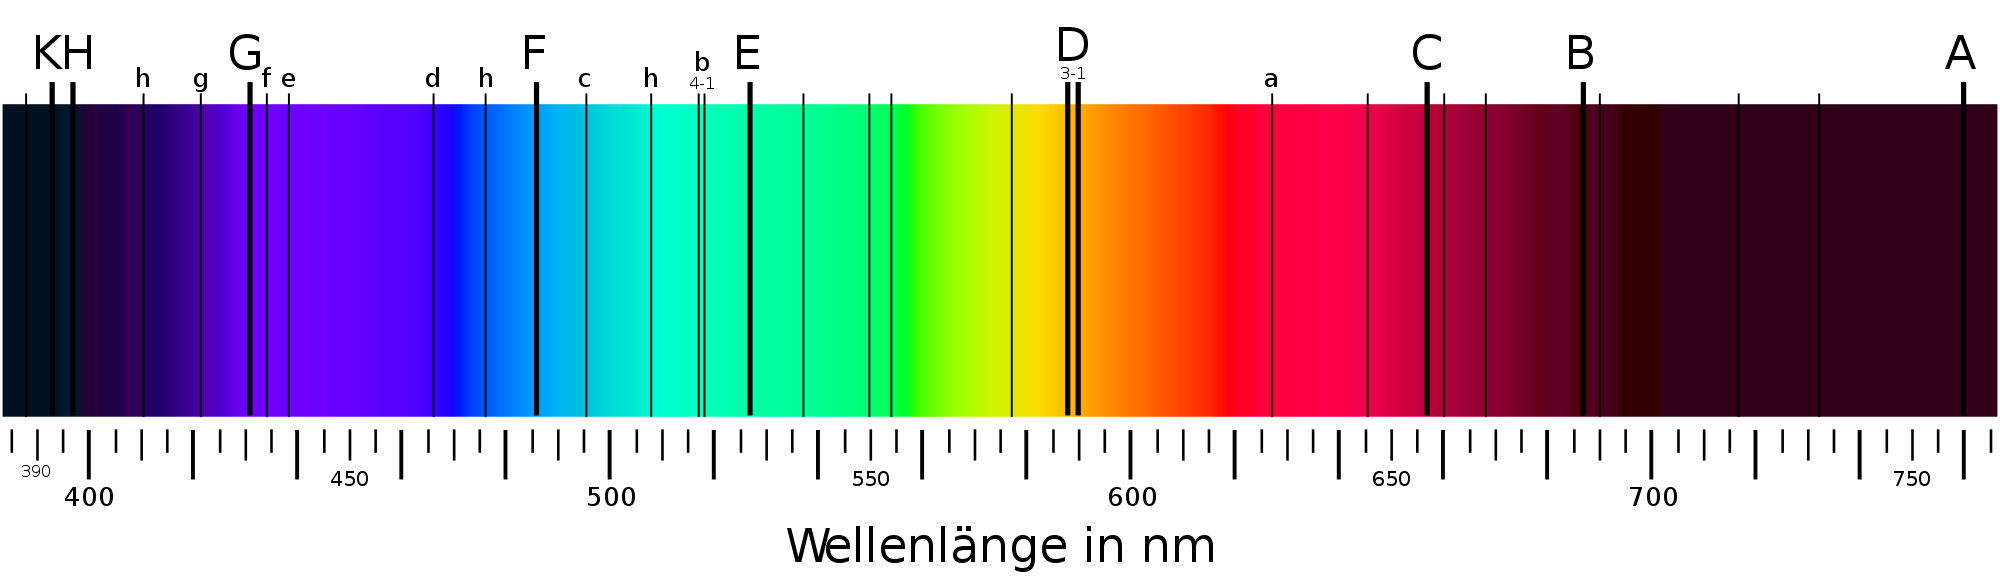
\includegraphics[width=0.8\textwidth]{fraunhofer_linien.png}
    \caption{Fraunhofer'sche Linien im Sonnenlichtspektrum}
    \label{fig:fraunhofer-linien}
\end{figure}

% 1.2.2 Entdeckung Bunsen, Kirchhoff
1859 führten Gustav Robert Kirchhoff und Robert Bunsen ein Experiment durch, bei dem eine Assoziazion zwischen chemischen Elementen und den Fraunhofer'schen Linien beobachtet wurde. Daraus folgt, dass die Absorptionslinien des Sonnenspektrums, welche Fraunhofer analysierte, die Absorptionseigenschaften dieser Elemente reflektieren.

\begin{wraptable}{l}{0pt}
    \label{tab:wichtige-fraunhoferlinien}
    \begin{tabular}{|c|c|c|}
        \hline
        Name & Element & Wellenlänge \\
        y    & $O_2$    & 898,765    \\
        Z    & $O_2$    & 822,696    \\
        ...  & ...      & ...        \\ % TODO ganze tabelle
        \hline
    \end{tabular}
    \caption{Wichtigste Fraunhofer'schen Linien}
\end{wraptable}

% 1.3 IR-Spektroskopie
% 1.3.1 Was ist es?
Bei der Infrarotspektroskopie werden Wellen im Infrarotbereich (ca. 800nm-1mm) zerlegt.

% 1.3.2 Vgl. Fraunhofer
Genau wie bei Fraunhofers Lichtspektrometer dient die Infrarotspektroskopie dem Nachweis chemischer Stoffe. Während das Lichtspektrometer die chemische Zusammensetzung der Sterne durch die Absorption am sichtbaren Licht der dortigen Elemente nachweist, kann das Infrarotlicht eines IR-Spektrometers Schwingungen in bestimmten chemischen Gruppen anregen, und somit in gewissen Wellenlängenbereichen Absorptionen herbeirufen.

% 1.3.3 Methoden: FTIR, Laser, Raman, ATR, etc.
Zu den arten der IR-Spektroskopie gehören u. A. FTIR-, Raman-, und ATR-Spektroskopie.

\newpage
\section{Theoretische Grundlagen}

% Übergang

\subsection{Interferenz}

% Warum Grundlage?

\subsection{Doppelspaltexperiment}

% Warum Grundlage?
% Verbindung zu Interferenz

\subsection{Absorption}

% Warum Grundlage?

\section{IR-Spektrometer}

% Übergang

\subsection{Komponenten}

\subsubsection{Strahlquelle}

% λ × T = b
% Lötkolben

\subsubsection{Abbildende Optik}

% Spiegel

\subsubsection{Gitter}

% 600 Linien / mm
% Leypold
% Reflexionsgitter

\section{Versuch und Ergebnisse}

% b = k × λ ÷ sin(α)
%   α = 30°; λ = 530nm
%   -> b = 1500nm

\subsection{Versuchsaufbau}

% Bilder:
%   - loetkolben
%   - hg-lampe
%   - spiegel
%   - sensor
%   - gitter

\subsection{Ergebnisse}

% Diagramme
% Fehler

\section{Arduino} % Später

\subsection{Motorsteuerung}

\subsection{Signalerfassung}

\end{document}